\documentclass[a4paper]{article}

\RequirePackage[T1,T2A]{fontenc}
\RequirePackage[utf8]{inputenc}
\RequirePackage[russian]{babel}

\RequirePackage[left=2cm,right=2cm, top=2cm,bottom=2cm,bindingoffset=0cm]{geometry}

\RequirePackage{amsmath}
\RequirePackage{amssymb}
\RequirePackage{amsfonts}
\RequirePackage{amsthm}

\RequirePackage{graphicx}
\RequirePackage{fancyhdr}
\RequirePackage{mathtools}
\RequirePackage{wrapfig}

\usepackage[colorlinks,citecolor=black,linkcolor=black,bookmarks=false,hypertexnames=true, urlcolor=blue]{hyperref}

\title{Отчёт по \href{https://github.com/ARS404/DiffusionProject}{проекту}}
\author{Зайцев Фёдор, Ознобихин Арсений}
\begin{document}
    \maketitle{}
    \tableofcontents
    \newpage

    \section{Постановка задачи}
    \subsection{Задача}
    Реализация 3 солвера ОДУ, порожденного диффузионной моделью (Эйлер, DDIM, EDM),
    и сравнение их качества.

    \subsection{Цели}
    \begin{itemize}
        \item Реализация солверов.
        \item Реализация необходимого для проведения экспериментов кода.
        \item Проведение экспериментов.
        \item Сравнение результатов
    \end{itemize}

    \subsection{Описание методов}

    \subsubsection{Диффузионная модель}
    В данной работе мы использовали диффузионную модель, обученную для выполнения задачи денойзера дифференциального уравнения со взрывающейся дисперсией, предсказывающего точку $X_0$ по входным данным $X_{\sigma}$ и дисперсии $\sigma$. Будем обозначать эту модель $D^{\theta}_{\sigma}(X_{\sigma})$. Мы сравнили несколько алгоритмов решения ОДУ при помощи данной модели, рассмотрим их далее. Для каждого алгоритма запишем один шаг генерации для момента i. Стоит учесть, что при сэмплировании мы будем итерироваться по i в порядке убывания от T к 0, где T - общее заданное количество шагов генерации.
    
    \subsubsection{Эйлер}
    Данный солвер реализовывал алгоритм построения исходных данных при помощи схемы Эйлера. Мы использовали ее для решения обратного ОДУ и, соответственно, применяли формулу дискретизации $\mathbf{Y}_{t - h} \approx  \mathbf{Y}_t + h \cdot t \cdot \nabla \log p_t(\mathbf{Y}_t)$. Выражая наш алгоритм через конкретные узлы дискретизации и применяя параметризацию через обученный денойзер мы имеем следующую формулу для ОДУ сэмплирования: 
    $$x_{i - 1} = x_{i} + (t_{i} - {t_{i-1}}) \cdot \frac{D^{\theta}_{t_{i}}(x_{i}) - x_{i}}{t_{i}}$$
    Данную схему генерации мы подробно обсуждали на семинарах и лекциях и интуиция за ней стоит довольно простая - мы просто дискретизуем обратное дифференциальное уравнение по схеме Эйлера.

    \subsubsection{EDM}

    Стохастический сэмплер с коррекцией направления второго порядка, предложенный в той же статье, что и EDM модель денойзера, применяет улучшенную схему Эйлера - Heun's 2nd order method, также известную как трапезоидальное правило. Данный метод заключается в оценке диффура в следующей точке дискретизации при помощи двух обращений к нашей функции оценки, вместо одного, по следующему правилу: 
    $$\hat{y}_{i + 1} = y_i + hf(t_i, y_i)$$

    $$y_{i+1} = y_{i} + \frac{h}{2}(f(t_i, y_i) + f(t_{i+1}, \hat{y}_{i + 1}))$$

    Авторы отмечают, что применение подобного метода позволяет улучшить качество сэмплирования, не так сильно при этом набрав в количестве обращений к нашей оценочной функции.

    Авторы статьи предлагают комбинировать использование данного метода вместе с добавлением дополнительной стохастичности посредством добавления и отнятия шума. Итого получаем следующий алгоритм:
    $$\hat{x}_i = x_i + \sqrt{((1 + \gamma_i)t_{i})^2 - t_i^2} \epsilon_i - \text{добавление нового шума}$$
    $$\hat{x}_{i - 1} = \hat{x}_{i} + (\hat{t}_{i} - {t_{i-1}}) \cdot \frac{D^{\theta}_{\hat{t}_{i}}(\hat{x}_{i}) - \hat{x}_{i}}{\hat{t}_{i}} - \text{первый шаг Эйлера}$$
    $$x_{i - 1} = \hat{x}_{i} + (\hat{t}_{i} - {t_{i-1}}) \cdot \frac12 (\frac{D^{\theta}_{\hat{t}_{i}}(\hat{x}_{i}) - \hat{x}_{i}}{\hat{t}_{i}} + \frac{D^{\theta}_{t_{i-1}}(\hat{x}_{i-1}) - \hat{x}_{i-1}}{t_{i-1}}) - \text{коррекция второго порядка}$$

    За стохастичность в данном алгоритме отвечают гиперпараметры $\gamma_i$ и случайно засэмплированные величины $\epsilon_i \sim \mathcal{N}(0, S^2_{noise} I)$

    Узлы дискретизации для этого метода, как и для предыдущего, выбирались с опорой на статью про модель EDM (оптимальные гиперпараметры со сглаженным переходом от $\sigma_{min}$ к $\sigma_{max}$ так же, как на семинаре.)

    \subsubsection{DDIM}

    Этот алгортим, в отличие от двух предыдущих, работает с дифференциальным уравнением с сохраняющейся дисперсией $X_t = \sqrt{\alpha_t}X_0 + \sqrt{1 - \alpha_t}\epsilon$. Соответственно нетрудно показать путем легких преобразований, что для получения оценки $\hat{X}_0$, нам нужно вычислить функцию $D^{\theta}_{\sqrt{\frac{1 - \alpha_t}{\alpha_t}}}(\frac{X_{t}}{\sqrt{\alpha_t}})$. Есть правда еще один нюанс - оригинальный алгоритм работает с моделью, параметризованной на оценку шума - разницы между $X_t$ и $X_0$, так что нам и здесь придется немного извернуться с формулами, оценив этот самый шум, как $\hat{\epsilon_t} = \frac{X_t - \hat{X}_0 \sqrt{\alpha_t}}{\sqrt{1 - \alpha_t}}$. Имея на руках наши оценки для шума и изначальной точки, мы можем выписать шаг DDIM, он будет выглядеть следующим образом:
    $$x_{i-1} = \sqrt{\alpha_{i-1}} \hat{x}_0 + \sqrt{1 - \alpha_{i-1}}\hat{\epsilon_i}$$

    Данный алгоритм является частным случаем более генерализованного стохастичного алгоритма, обобщающего генерацию для не-Марковских процессов. Обнуление в этом процессе коэффициента, отвечающего за добавление шума на каждом шаге генерации, и дает нам данный алгоритм.

    Узлы дискретизации для этого метода выбирались исходя из результатов в соответствующей работе - наилучшего качества авторам удалось добиться для квадратичного расписания $\beta_{t}$.

    \section{Техническое описание экспериментов}
    Все эксперименты проводились на датасете CIFAR-10, в качестве диффузионной модели была использована модель, предложенная в статье по EDM, обученная на датасете CIFAR-10 для необусловленной генерации с помощью VE диффура (получена по \href{https://nvlabs-fi-cdn.nvidia.com/edm/pretrained/}{ссылке}).
    Для каждого из реализованных солверов было проведено несколько экспериментов по генерации и подсчету FID скора. Мы сравнивали между собой работу алгоритмов при количестве шагов генерации 50 и 200. Для этих значений FID скор подсчитывался на 3000 сгенерированных изображениях. Также мы подсчитывали FID скор для 5000 изображений при 100 шагах генерации для каждого солвера. Далее проводилось количественное (по FID) и качественное (визуально) сравнение результатов.

    Остальные гиперпараметры (настройки стохастичности в EDM) выставлялись в соответствии с оптимальными гиперпараметрами, описанными в статьях.
    
    \par Более подробное описание процесса запуска экспериментов можно увидеть в
    \href{https://github.com/ARS404/DiffusionProject}{README}

    Запуск экспериментов занимал разное количество времени от 10 минут (50-шаговая генерация 3000 изображений Эйлером), до нескольких часов (генерация 1000 шагов DDIM для 3000 изображений).


    \section{Результаты экспериментов}
    \subsection{Описание результатов}
    
    Было проведено несколько экспериментов, с различным количеством шагов солверов:
    \begin{table}
        \centering
        \begin{tabular}{ l | c | c | c }
            \textbf{Solver} & Euler & DDIM  & EDM \\ \hline
            \textbf{FID}    & 11{,}55 & 354{,}51 & 10{,}68
        \end{tabular}\hspace{50pt}%
        \begin{tabular}{ l | c | c | c | c }
            \textbf{Solver} & Euler & DDIM  & EDM \\ \hline
            \textbf{FID}    & 10{,}96 & 152{,}53 & 11{,}39
        \end{tabular}
        \caption{Для 50 (слева) и 200 (справа) степов и 3000 семплов}
        \label{tab:tab1}
    \end{table}
    \begin{table}
        \centering
        \begin{tabular}{ l | c | c | c }
            \textbf{Solver} & Euler & DDIM  & EDM \\ \hline
            \textbf{FID}    & 7{,}59 & 321{,}57 & 7{,}19 
        \end{tabular}
        \caption{Для 100 степов и 5000 семплов}
        \label{tab:tab2}
    \end{table}
    \begin{table}
        \centering
        \begin{tabular}{ l | c | c | c | c }
            \textbf{Steps} & 50 & 200 & 500 & 1000 \\ \hline
            \textbf{FID}   & 354{,}51 & 152{,}53 & 18{,}61 & 11{,}24
        \end{tabular}
        \caption{Результаты DDIM в зависимости от количества шагов}
        \label{tab:tab3}
    \end{table}

    Кроме сравнения методов между собой (таб.~\ref{tab:tab1}), мы также убедились в том, что увеличение количества сэмплов для подсчета FID благоприятно влияет на скор (что также было отмечено в других экспериментах как с другими моделями и датасетами, так и с \href{https://github.com/yuanzhi-zhu/mini_edm}{нашими}) (таб.\ref{tab:tab2}) и запустили наиболее оптимальные количества степов (из оригинальных статей) для DDIM (1000 с FID = 11{,}24) и EDM (256 с FID = 11{,}57).
    \par Для визуального сравнения результатов мы прилагаем примеры сгенерированных изображений для лучшего конфига для каждого из солверов (их можно посмотреть в конце отчёта).
    
    \subsection{Анализ результатов}
    Наши эксперименты показали, что при работе с моделью EDM сопоставимое между собой качество дают солверы Эйлер и EDM. При одинаковом количестве итераций они давали близкие значения FID во всех сеттингах. Стоит однако отметить, что метод генерации EDM второго порядка потребляет заметно большее количество вычислительных ресурсов, так как на каждом шаге итерации ему нужно дважды посчитать выход модели, а Эйлеровской схеме - лишь раз. Вследствие чего можно сделать вывод о том, что схема Эйлера при сравнимом качестве генерации является более эффективным подходом при учете затраченных вычислительных ресурсов. Компенсирует этот недостаток алгоритм EDM своей дополнительной стохастичностью - при помощи введения дополнительного шума он имеет возможность генерировать более разнообразные сэмплы, чем алгоритм генерации по Эйлеру.
    Что касается алгоритма DDIM, эксперименты показали, что ему нужно наибольшее количество шагов для схождения к адекватному результату. При этом он способен показывать сопоставимое качество, но просто за гораздо большее время (именно за счёт необходимости использовать б\`{о}льшее количество степов). Для 1000 шагов генерации DDIM показывал качество на уровне с 50-200 шагами генерации EDM или Эйлеровского алгоритма (таб.~\ref{tab:tab3}).
    \par Визуальный анализ также позволяет убедиться в том, что все солверы при оптимальных настройках гиперпараметров показывают сравнимое между собой относительно неплохое качество. Можно убедиться <<методом пристального взгляда>> в том, что сгенерированные сэмплы достаточно разнообразны и отражают все классы датасета, выдавая терпимое качество, но не всегда избегая некоторых огрехов, артефактов, зашумленностей и нереалистичных деталей.
    
    \section{Вывод}
    По результатам экспериментов среди предложенных методов наименее применимым оказался метод DDIM - он работает значительно дольше других двух методов, не оправдывая это значительно более лучшим качеством. Методы Эйлера и EDM могут быть успешно применены в разных ситуациях, например метод Эйлера может быть более успешен в случае ограниченности вычислительных ресурсов, так как задействует заметно меньшее количество таковых, а метод EDM может быть использован в случаях, когда нам нужно добиться большей стохастичности генерации, так как он содержит в себе двойное применение схемы Эйлера (каждое из которых можно обратить в стохастичное) и также дополнительный шум, позволяющий добиться большего разнообразия в генерации.

    Резюмируя вышенаписанное, в ходе выполнения проекта нам удалось достичь поставленных целей и, несмотря на достаточно большие значения FID, получить достаточно естественно выглядящие изображения в разрешении $32 \times 32$ на которых чётко прослеживаются классы, которые содержатся в датасете CIFAR-10.
    \par В целом, результаты нашей работы показывают, что рассмотренные решения достаточно хорошо подходят для датасетов в маленьком разрешении, и два из них работают достаточно быстро. Тем не менее, интересно было бы проверить качество решений и на других датасетах большего разрешения, а также сравнить FID для большего количества сгенерированных сэмплов.

    \section{Разделение работы}
    \begin{itemize}
        \item Реализация солверов:
            \begin{itemize}
                \item Euler --- Фёдор (ред. Арсений);
                \item DDIM --- Фёдор (ред. Арсений);
                \item EDM --- Арсений (ред. Фёдор);
            \end{itemize}
        \item Составление архитектуры --- совместно;
        \item Реализация общего для всех солверов кода --- Арсений (ред. Фёдор);
        \item Создание и оформление репозитория --- Арсений (ред. Фёдор);
        \item Проведение экспериментов --- совместно;
        \item Составление отчёта --- совместно.
    \end{itemize}

    \newpage
    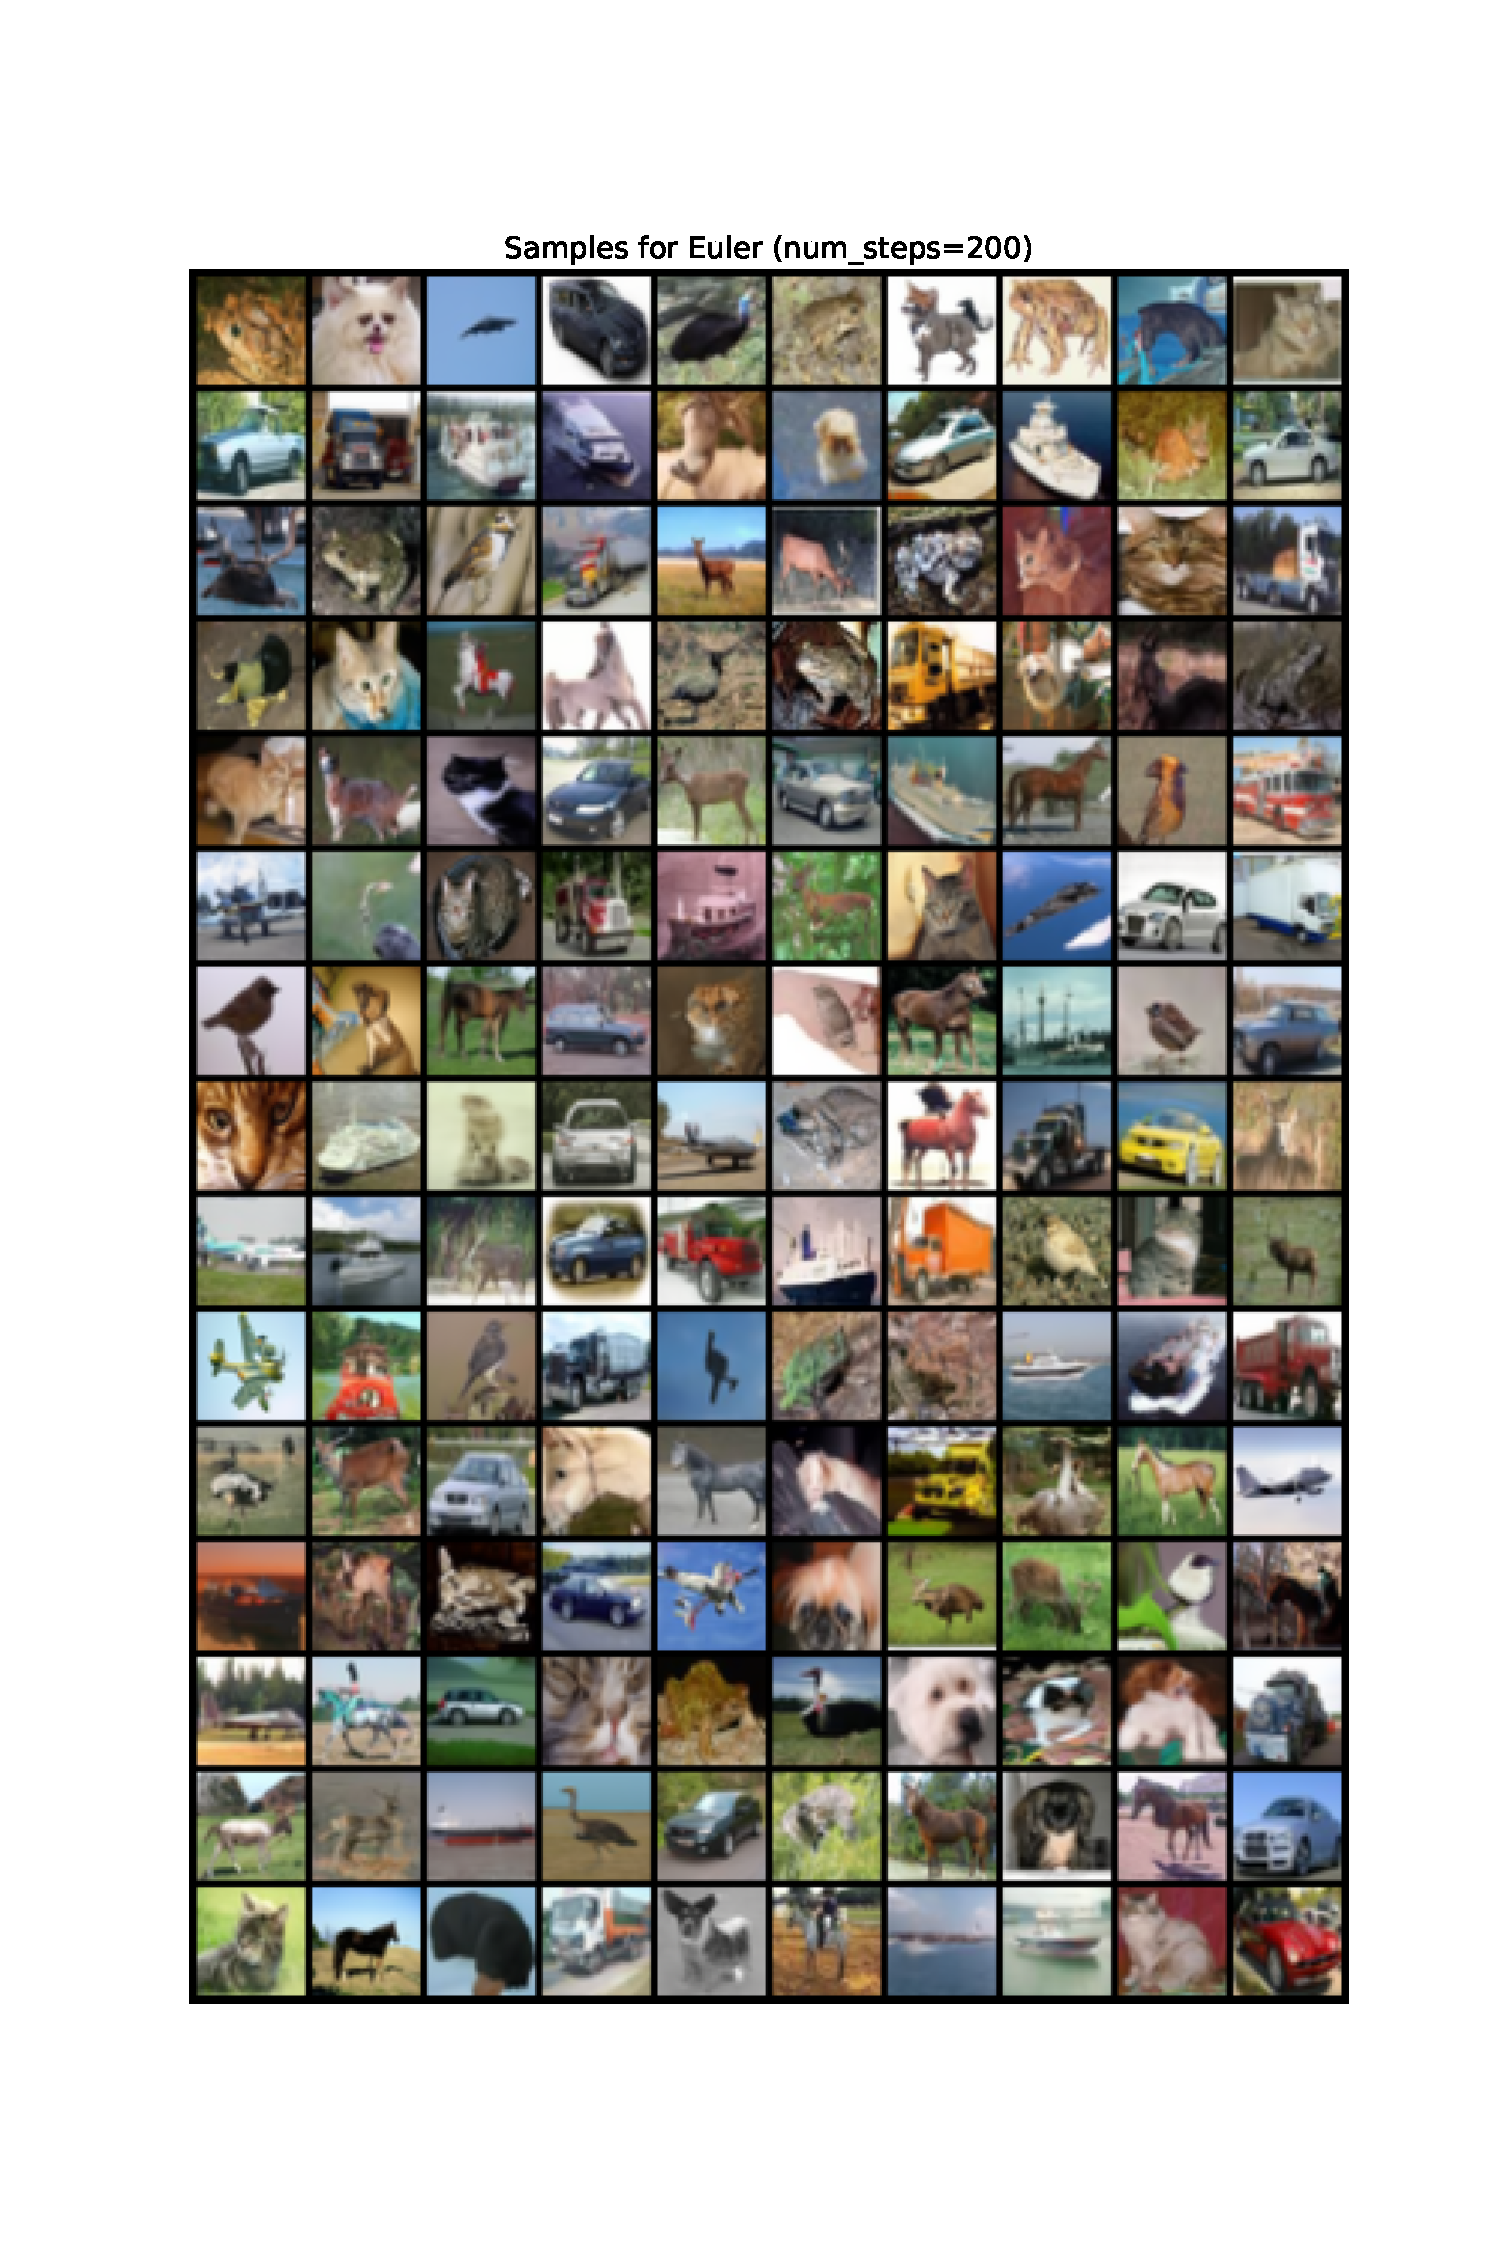
\includegraphics[width=0.98\textwidth]{data/Samples_for_Euler_(num_steps=200).pdf}
    \newpage
    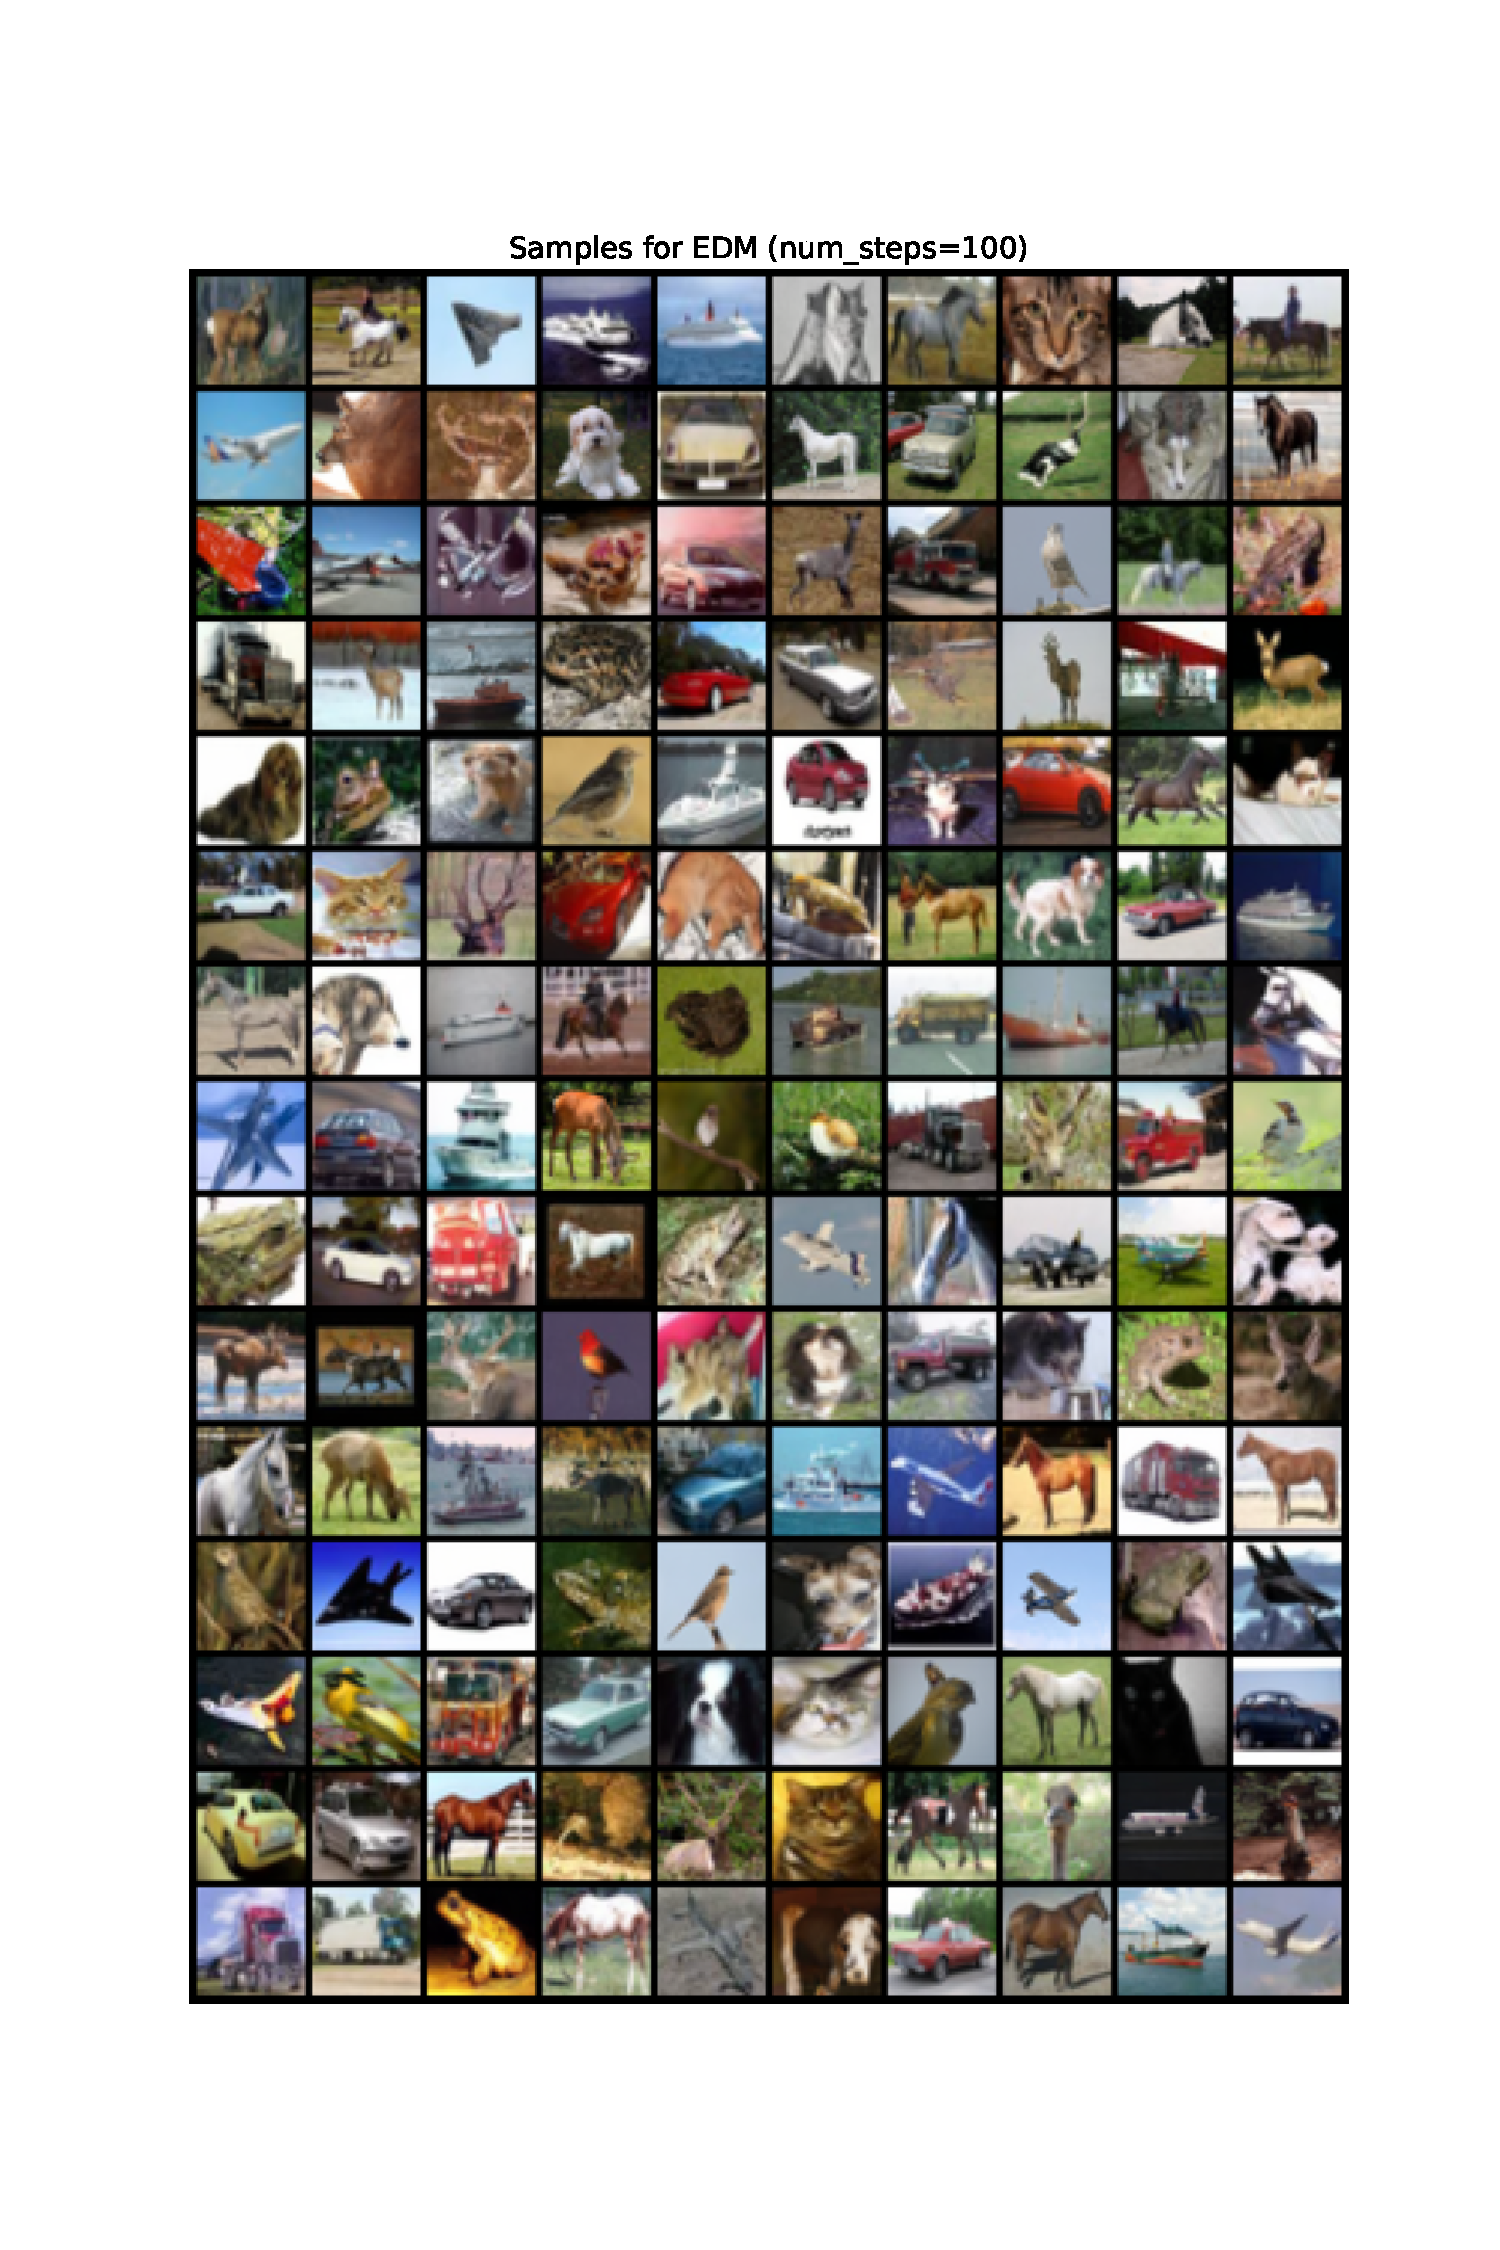
\includegraphics[width=0.98\textwidth]{data/Samples_for_EDM_(num_steps=100).pdf}
    \newpage
    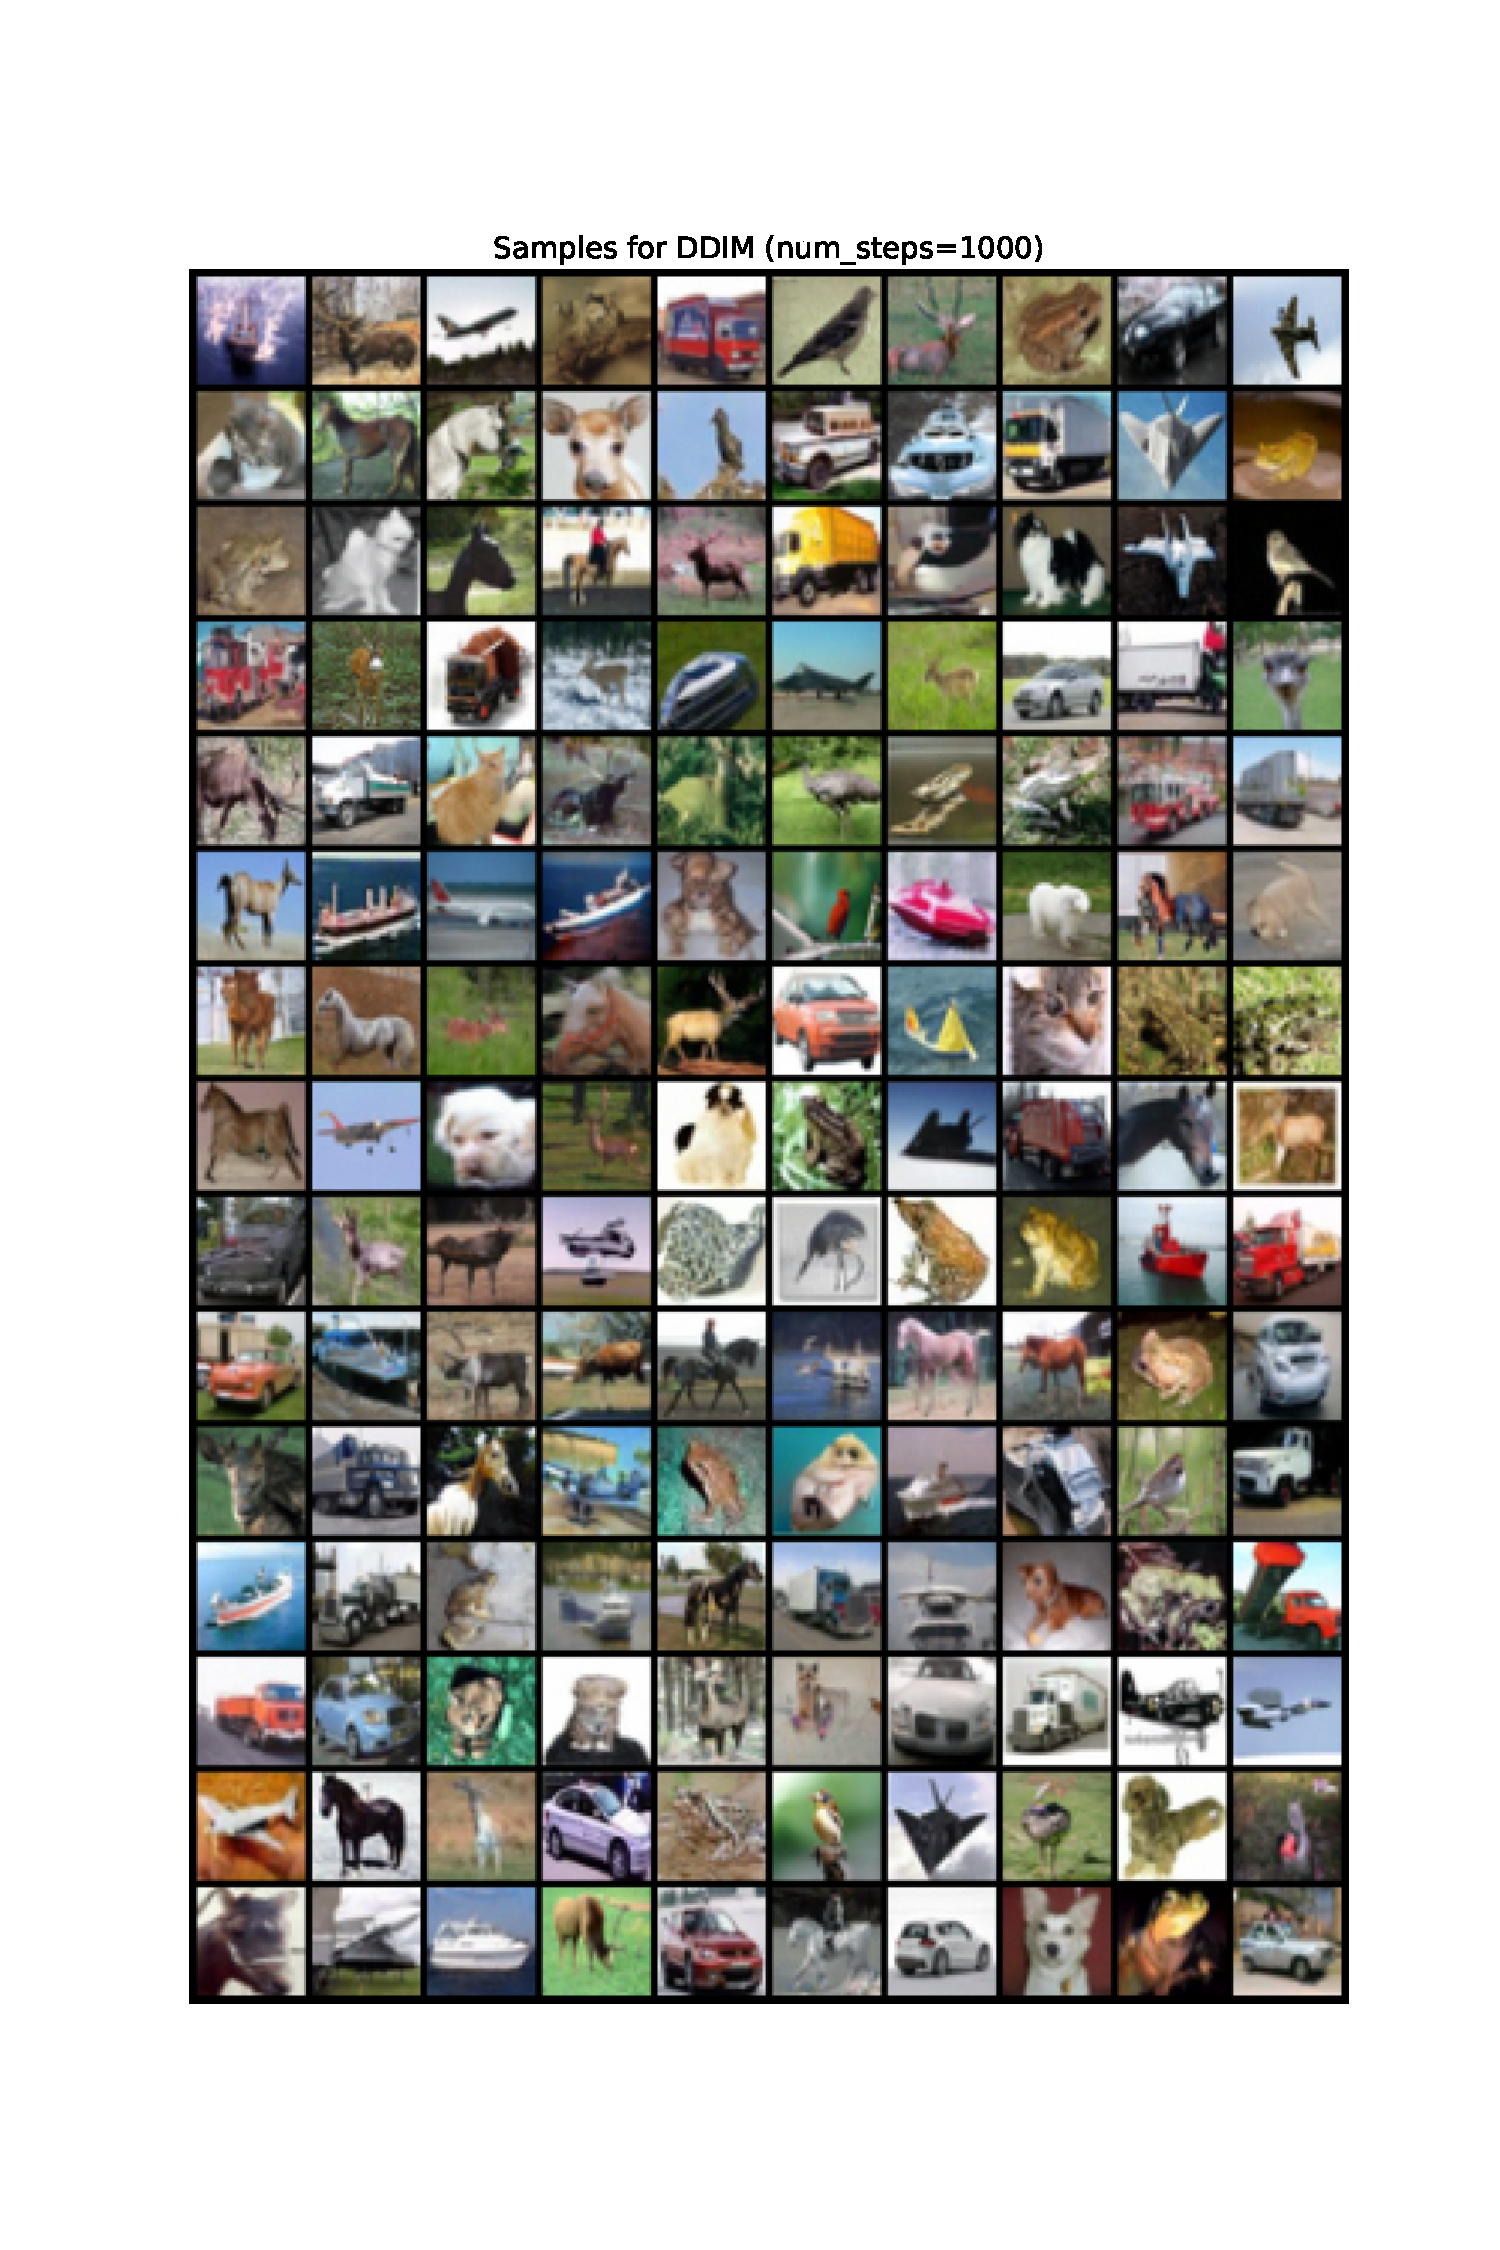
\includegraphics[width=0.98\textwidth]{data/Samples_for_DDIM_(num_steps=1000).pdf}
\end{document}